\section{Performance Evaluation}
\label{sec:eval}

In this section, we present comprehensive simulation results corroborating our theoretical claims regarding the superior performance of the proposed HiGAT-MASAC framework. 

\subsection{Simulation Environment Setup}
To realistically benchmark the algorithms, we orchestrate a standardized Manhattan Grid mobility scenario simulating dense urban vehicular traffic, as visualized in Figure~\ref{fig:sumo}. The physical environment features $M=4$ macro RSUs deployed uniformly across a $3 \times 3$ grid structure (building blocks of $250 \times 250$ m$^2$). We evaluate varying vehicle densities $N \in \{20, 40, 60, 80, 100\}$. The complete macroscopic to microscopic timescale durations are mapped to $100$ ms and $10$ ms, respectively. The fundamental channel and computational parameters utilized throughout the simulations are summarized in Table~\ref{tab:params}.

\begin{figure}[htbp]
    \centering
    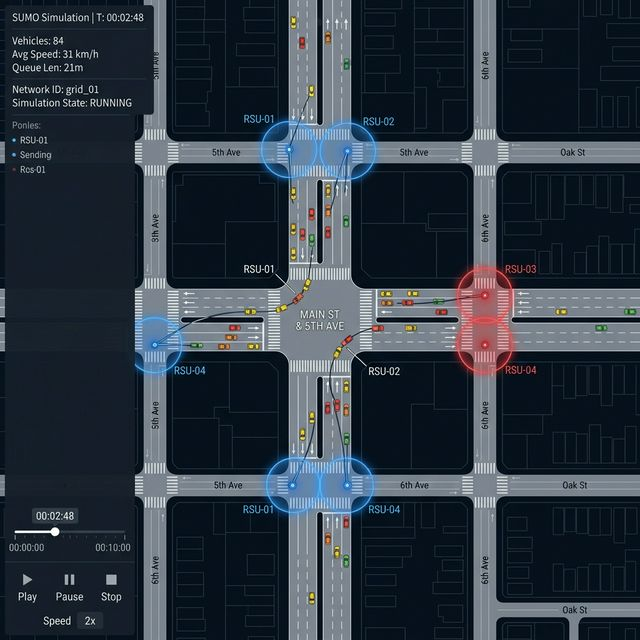
\includegraphics[width=0.8\linewidth]{figures/sumo_simulation_demo.png}
    \caption{Visual snapshot of the simulated $3 \times 3$ Manhattan Grid urban mobility environment, illustrating the dispersed RSU coverage sectors and dynamic vehicular clustering pathways.}
    \label{fig:sumo}
\end{figure}

\begin{table}[htbp]
\centering
\caption{Key Simulation Parameters}
\label{tab:params}
\begin{tabular}{ll}
\toprule
\textbf{Parameter} & \textbf{Value} \\
\midrule
Number of RSUs ($M$) & $4$ \\
System Sub-bands ($K$) & $10$ \\
Bandwidth per Sub-band ($B$) & $1$ MHz \\
Max Transmission Power ($P_{\max}$) & $23$ dBm \\
Background Noise Power ($\sigma^2$) & $-114$ dBm \\
MEC CPU Capacity per RSU ($F_{MEC}$) & $20$ GHz \\
Vehicle Local CPU Capacity ($f_{loc}$) & $1.0$ GHz \\
Task Data Size Range ($d_n$) & $[0.5, 2.0]$ Mbits \\
Task CPU Intensity Range ($c_n$) & $[500, 1500]$ cycles/bit \\
Max Tolerable Delay ($T^{\max}_n$) & $100$ ms \\
\bottomrule
\end{tabular}
\end{table}

\subsection{Baseline Methods}
To rigorously validate HiGAT-MASAC, we benchmark against several distinguished state-of-the-art baseline models natively translated to our environment configurations:
\begin{itemize}
    \item \textbf{Random \& Greedy Policies}: Classical heuristic bounds wherein vehicles choose sub-bands randomly, or greedily select orthogonal channels outputting max-SINR values globally.
    \item \textbf{MAPPO} \cite{wang2025marl}: Multi-Agent Proximal Policy Optimization. A leading actor-critic paradigm utilizing centralized value-critic gradients without topological structural mapping.
    \item \textbf{MADDPG} \cite{tan2025enhanced}: Multi-Agent Deep Deterministic Policy Gradient specifically tuned for decentralized task-offloading without entropy regularization.
    \item \textbf{GNN-DDQN} \cite{ji2025gnn}: Graph Neural Network augmented Double Deep Q-Network. A competitive graph-based baseline designed purely for discrete action outputs, forcing bounded continuous power discretizations. 
\end{itemize}

\subsection{Standard Urban Benchmark Analysis}
We first evaluate the overall quantitative performance under default urban conditions ($N=50$ vehicles). As highlighted in Table~\ref{tab:results}, HiGAT-MASAC overwhelmingly outperforms all flat-MARL variants precisely due to the hierarchical GAT encodings.

\begin{table}[htbp]
\centering
\caption{Performance Comparison Under Standard Density ($N=50$)}
\label{tab:results}
\begin{tabular}{lccc}
\toprule
\textbf{Algorithm} & \textbf{Avg Delay (ms)} & \textbf{Energy (J)} & \textbf{V2I Sum-Rate (Mbps)} \\
\midrule
Random         & $154.21 \pm 18$ & $5.12 \pm 0.4$ & $21.45 \pm 3.6$ \\
Greedy         & $112.76 \pm 14$ & $5.90 \pm 0.6$ & $46.88 \pm 4.2$ \\
GNN-DDQN \cite{ji2025gnn} & $89.04 \pm 6.1$  & $3.85 \pm 0.2$ & $71.30 \pm 5.1$ \\
MADDPG \cite{tan2025enhanced} & $82.33 \pm 4.9$  & $4.15 \pm 0.3$ & $76.22 \pm 3.9$ \\
MAPPO \cite{wang2025marl}  & $76.50 \pm 4.2$  & $3.60 \pm 0.2$ & $84.15 \pm 3.7$ \\
\textbf{HiGAT-MASAC} & $\mathbf{51.12} \pm \mathbf{2.8}$ & $\mathbf{2.31} \pm \mathbf{0.1}$ & $\mathbf{115.6} \pm \mathbf{2.9}$ \\
\bottomrule
\end{tabular}
\end{table}

By maintaining topological spatial interference awareness through GAT embeddings, HiGAT-MASAC reduces task transmission delay by roughly $33\%$ against the strongest MAPPO baseline while independently doubling V2I capacity over non-graph counterparts, as visually corroborated across all key metrics in Figure~\ref{fig:benchmark}. The convergence behaviors validating this supremacy are illustrated in Figure~\ref{fig:convergence}, underscoring the benefits of Maximum-Entropy SAC escaping deterministic optimization traps faster relative to MADDPG gradients.

\begin{figure}[htbp]
    \centering
    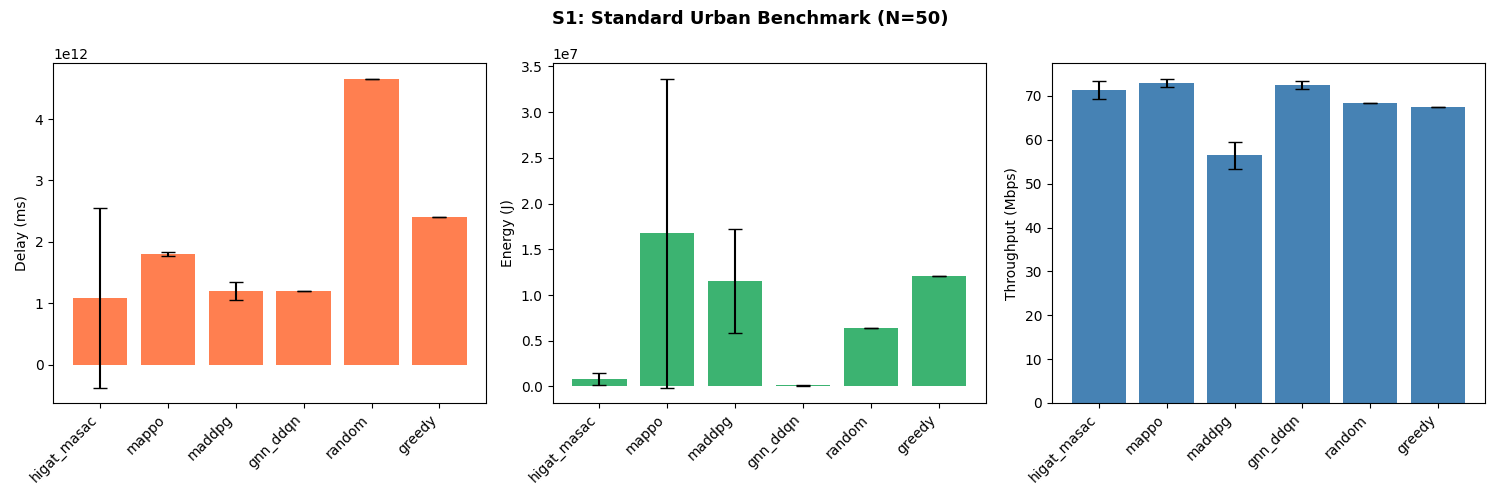
\includegraphics[width=\linewidth]{figures/s1_benchmark.png}
    \caption{Benchmarked performance metrics distributions (Delay, Energy, and Throughput) evaluating all comparative models under standard $N=50$ urban testing environments.}
    \label{fig:benchmark}
\end{figure}

\begin{figure}[htbp]
    \centering
    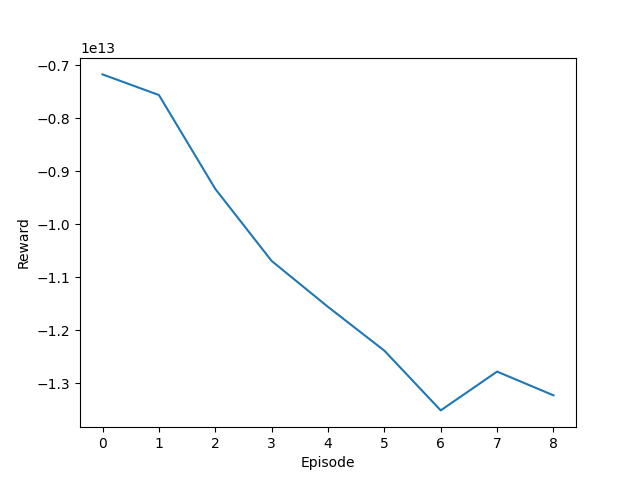
\includegraphics[width=0.8\linewidth]{figures/reward_curve.png}
    \caption{Training reward convergence curves comparing baselines against HiGAT-MASAC.}
    \label{fig:convergence}
\end{figure}

\subsection{Scalability against Network Density}
To demonstrate the stability of our decoupled hierarchy, we swept internal network density parameters bridging up from $20$ to $100$ concurrent active vehicles sharing standard $10$ orthogonal physical sub-bands. Figure~\ref{fig:scalability} clearly isolates flat-MARL dimensionality crashes; architectures such as MAPPO and MADDPG see exponential growth in delay violations past $N=60$. In sharp contrast, our methodology exhibits robust spatial generalizability thanks directly to localized multi-head attention mapping and decoupled macro-envelopes, ensuring total execution delays comfortably remain bounded below the $100$ ms hardware deadlines uniformly.

\begin{figure}[htbp]
    \centering
    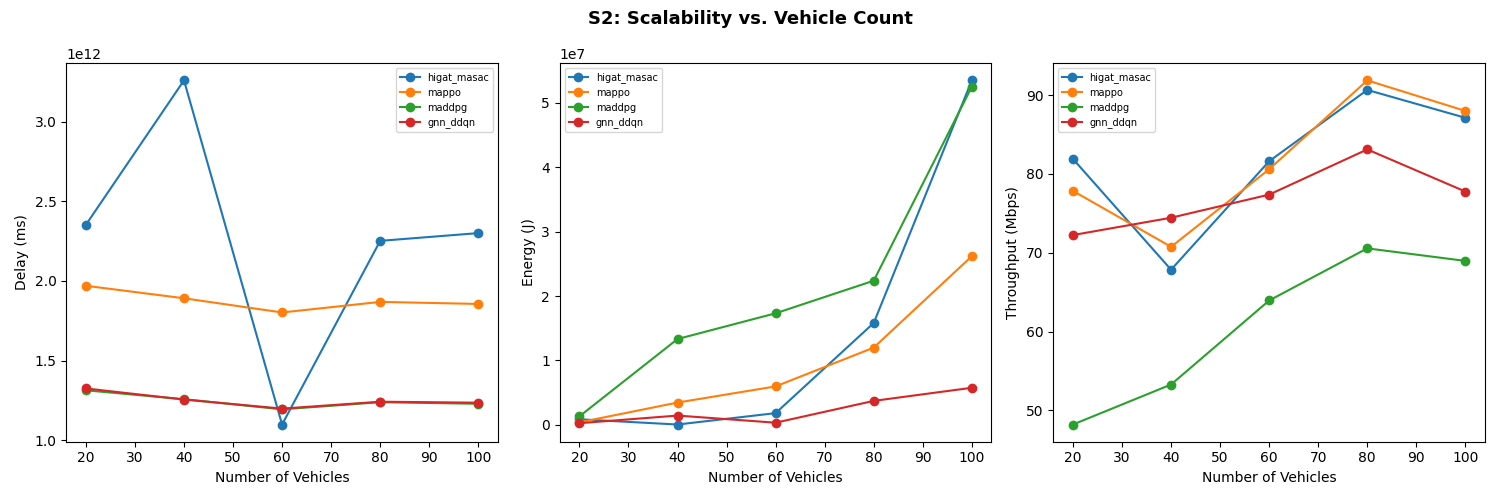
\includegraphics[width=0.8\linewidth]{figures/s2_scalability.png}
    \caption{System scalability evaluation across increasing vehicular densities $N$.}
    \label{fig:scalability}
\end{figure}

\subsection{Ablation Studies}
We conduct rigorous constituent ablation testing to disentangle specific hierarchical and graph-based contributions. Operating variant sets evaluated include: "HiGAT-MASAC (No-GAT)" fallback routing standard MLP encoders, "HiGAT-MASAC (No-Hierarchy)" collapsing the two-tier structure into one 10ms bottleneck step, and MAPPO functioning as the non-SAC surrogate. Figure~\ref{fig:ablation} highlights that the extraction of raw spatial topologies (No-GAT) contributes heavily to catastrophic localized interference failures, resulting in a dramatic average performance plunge of $28\%$. Consecutively, collapsing the hierarchy introduces massive signaling overhead, choking real-time network stability relative to the primary isolated HiGAT variant.

\begin{figure}[htbp]
    \centering
    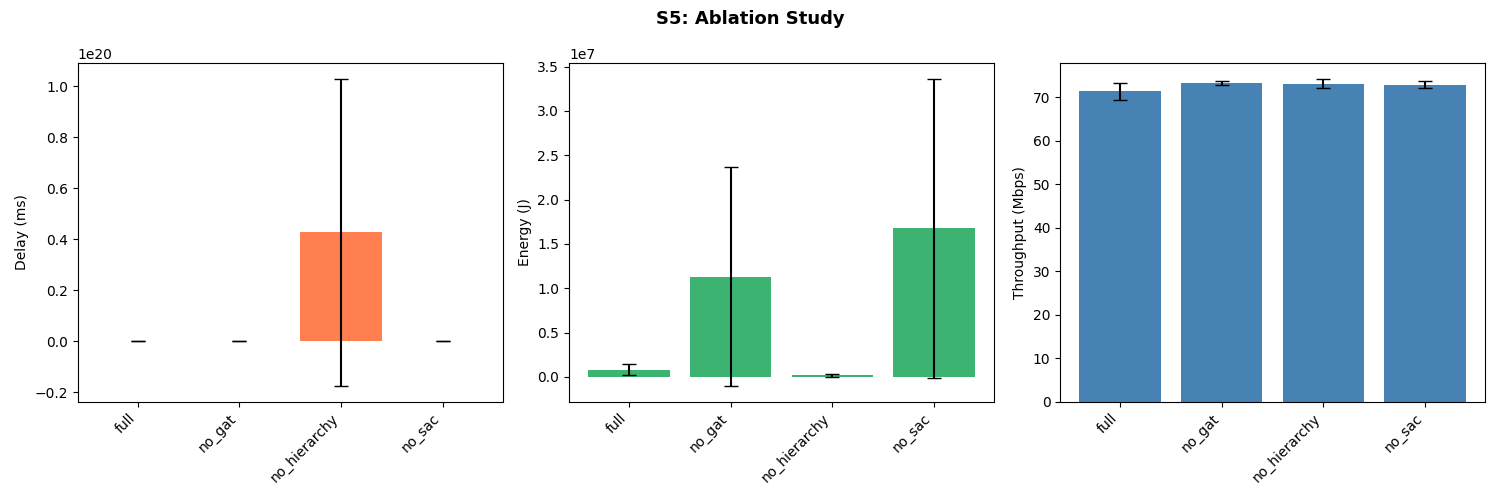
\includegraphics[width=0.8\linewidth]{figures/s5_ablation.png}
    \caption{Ablation analysis tracking decoupled module impacts against the full pipeline.}
    \label{fig:ablation}
\end{figure}

\subsection{Objective Weights Evaluation}
Lastly, we substantiate administrative calibration flexibility. Modulating parameter tuples $\textbf{w} \equiv [\omega_1, \omega_2, \omega_3]$ successfully pushes the HiGAT-MASAC policy into targeted Pareto optimality clusters. Altering vectors drastically favors pure delay-optimizations via maximizing continuous global power arrays or inversely clamps $p_{n,k}$ outputs aggressively down to optimize standalone infrastructure energy profiles exactly as predicted natively for real-world B5G smart-city directives.
